\documentclass[12pt,]{krantz}
\usepackage{lmodern}
\usepackage{amssymb,amsmath}
\usepackage{ifxetex,ifluatex}
\usepackage{fixltx2e} % provides \textsubscript
\ifnum 0\ifxetex 1\fi\ifluatex 1\fi=0 % if pdftex
  \usepackage[T1]{fontenc}
  \usepackage[utf8]{inputenc}
\else % if luatex or xelatex
  \ifxetex
    \usepackage{mathspec}
  \else
    \usepackage{fontspec}
  \fi
  \defaultfontfeatures{Ligatures=TeX,Scale=MatchLowercase}
    \setmonofont[Mapping=tex-ansi,Scale=0.7]{Source Code Pro}
\fi
% use upquote if available, for straight quotes in verbatim environments
\IfFileExists{upquote.sty}{\usepackage{upquote}}{}
% use microtype if available
\IfFileExists{microtype.sty}{%
\usepackage{microtype}
\UseMicrotypeSet[protrusion]{basicmath} % disable protrusion for tt fonts
}{}
\usepackage[unicode=true]{hyperref}
\PassOptionsToPackage{usenames,dvipsnames}{color} % color is loaded by hyperref
\hypersetup{
            pdftitle={Statistical Genetics: Analyses with R},
            pdfauthor={Dr.~Shirin Glander},
            colorlinks=true,
            linkcolor=Maroon,
            citecolor=Blue,
            urlcolor=Blue,
            breaklinks=true}
\urlstyle{same}  % don't use monospace font for urls
\usepackage{natbib}
\bibliographystyle{apalike}
\usepackage{color}
\usepackage{fancyvrb}
\newcommand{\VerbBar}{|}
\newcommand{\VERB}{\Verb[commandchars=\\\{\}]}
\DefineVerbatimEnvironment{Highlighting}{Verbatim}{commandchars=\\\{\}}
% Add ',fontsize=\small' for more characters per line
\usepackage{framed}
\definecolor{shadecolor}{RGB}{248,248,248}
\newenvironment{Shaded}{\begin{snugshade}}{\end{snugshade}}
\newcommand{\KeywordTok}[1]{\textcolor[rgb]{0.27,0.27,0.27}{\textbf{{#1}}}}
\newcommand{\DataTypeTok}[1]{\textcolor[rgb]{0.27,0.27,0.27}{{#1}}}
\newcommand{\DecValTok}[1]{\textcolor[rgb]{0.06,0.06,0.06}{{#1}}}
\newcommand{\BaseNTok}[1]{\textcolor[rgb]{0.06,0.06,0.06}{{#1}}}
\newcommand{\FloatTok}[1]{\textcolor[rgb]{0.06,0.06,0.06}{{#1}}}
\newcommand{\ConstantTok}[1]{\textcolor[rgb]{0,0,0}{{#1}}}
\newcommand{\CharTok}[1]{\textcolor[rgb]{0.5,0.5,0.5}{{#1}}}
\newcommand{\SpecialCharTok}[1]{\textcolor[rgb]{0,0,0}{{#1}}}
\newcommand{\StringTok}[1]{\textcolor[rgb]{0.5,0.5,0.5}{{#1}}}
\newcommand{\VerbatimStringTok}[1]{\textcolor[rgb]{0.5,0.5,0.5}{{#1}}}
\newcommand{\SpecialStringTok}[1]{\textcolor[rgb]{0.5,0.5,0.5}{{#1}}}
\newcommand{\ImportTok}[1]{{#1}}
\newcommand{\CommentTok}[1]{\textcolor[rgb]{0.37,0.37,0.37}{\textit{{#1}}}}
\newcommand{\DocumentationTok}[1]{\textcolor[rgb]{0.37,0.37,0.37}{\textbf{\textit{{#1}}}}}
\newcommand{\AnnotationTok}[1]{\textcolor[rgb]{0.37,0.37,0.37}{\textbf{\textit{{#1}}}}}
\newcommand{\CommentVarTok}[1]{\textcolor[rgb]{0.37,0.37,0.37}{\textbf{\textit{{#1}}}}}
\newcommand{\OtherTok}[1]{\textcolor[rgb]{0.37,0.37,0.37}{{#1}}}
\newcommand{\FunctionTok}[1]{\textcolor[rgb]{0,0,0}{{#1}}}
\newcommand{\VariableTok}[1]{\textcolor[rgb]{0,0,0}{{#1}}}
\newcommand{\ControlFlowTok}[1]{\textcolor[rgb]{0.27,0.27,0.27}{\textbf{{#1}}}}
\newcommand{\OperatorTok}[1]{\textcolor[rgb]{0.43,0.43,0.43}{\textbf{{#1}}}}
\newcommand{\BuiltInTok}[1]{{#1}}
\newcommand{\ExtensionTok}[1]{{#1}}
\newcommand{\PreprocessorTok}[1]{\textcolor[rgb]{0.37,0.37,0.37}{\textit{{#1}}}}
\newcommand{\AttributeTok}[1]{\textcolor[rgb]{0.61,0.61,0.61}{{#1}}}
\newcommand{\RegionMarkerTok}[1]{{#1}}
\newcommand{\InformationTok}[1]{\textcolor[rgb]{0.37,0.37,0.37}{\textbf{\textit{{#1}}}}}
\newcommand{\WarningTok}[1]{\textcolor[rgb]{0.37,0.37,0.37}{\textbf{\textit{{#1}}}}}
\newcommand{\AlertTok}[1]{\textcolor[rgb]{0.33,0.33,0.33}{{#1}}}
\newcommand{\ErrorTok}[1]{\textcolor[rgb]{0.14,0.14,0.14}{\textbf{{#1}}}}
\newcommand{\NormalTok}[1]{{#1}}
\usepackage{longtable,booktabs}
\usepackage{graphicx,grffile}
\makeatletter
\def\maxwidth{\ifdim\Gin@nat@width>\linewidth\linewidth\else\Gin@nat@width\fi}
\def\maxheight{\ifdim\Gin@nat@height>\textheight\textheight\else\Gin@nat@height\fi}
\makeatother
% Scale images if necessary, so that they will not overflow the page
% margins by default, and it is still possible to overwrite the defaults
% using explicit options in \includegraphics[width, height, ...]{}
\setkeys{Gin}{width=\maxwidth,height=\maxheight,keepaspectratio}
\IfFileExists{parskip.sty}{%
\usepackage{parskip}
}{% else
\setlength{\parindent}{0pt}
\setlength{\parskip}{6pt plus 2pt minus 1pt}
}
\setlength{\emergencystretch}{3em}  % prevent overfull lines
\providecommand{\tightlist}{%
  \setlength{\itemsep}{0pt}\setlength{\parskip}{0pt}}
\setcounter{secnumdepth}{5}
% Redefines (sub)paragraphs to behave more like sections
\ifx\paragraph\undefined\else
\let\oldparagraph\paragraph
\renewcommand{\paragraph}[1]{\oldparagraph{#1}\mbox{}}
\fi
\ifx\subparagraph\undefined\else
\let\oldsubparagraph\subparagraph
\renewcommand{\subparagraph}[1]{\oldsubparagraph{#1}\mbox{}}
\fi
\usepackage{booktabs}
\usepackage{longtable}
\usepackage[bf,singlelinecheck=off]{caption}

\usepackage{framed,color}
\definecolor{shadecolor}{RGB}{248,248,248}

\setmainfont[
  UprightFeatures={SmallCapsFont=AlegreyaSC-Regular}
]{Alegreya}

\renewcommand{\textfraction}{0.05}
\renewcommand{\topfraction}{0.8}
\renewcommand{\bottomfraction}{0.8}
\renewcommand{\floatpagefraction}{0.75}

\renewenvironment{quote}{\begin{VF}}{\end{VF}}
\let\oldhref\href
\renewcommand{\href}[2]{#2\footnote{\url{#1}}}

\ifxetex
  \usepackage{letltxmacro}
  \setlength{\XeTeXLinkMargin}{1pt}
  \LetLtxMacro\SavedIncludeGraphics\includegraphics
  \def\includegraphics#1#{% #1 catches optional stuff (star/opt. arg.)
    \IncludeGraphicsAux{#1}%
  }%
  \newcommand*{\IncludeGraphicsAux}[2]{%
    \XeTeXLinkBox{%
      \SavedIncludeGraphics#1{#2}%
    }%
  }%
\fi

\makeatletter
\newenvironment{kframe}{%
\medskip{}
\setlength{\fboxsep}{.8em}
 \def\at@end@of@kframe{}%
 \ifinner\ifhmode%
  \def\at@end@of@kframe{\end{minipage}}%
  \begin{minipage}{\columnwidth}%
 \fi\fi%
 \def\FrameCommand##1{\hskip\@totalleftmargin \hskip-\fboxsep
 \colorbox{shadecolor}{##1}\hskip-\fboxsep
     % There is no \\@totalrightmargin, so:
     \hskip-\linewidth \hskip-\@totalleftmargin \hskip\columnwidth}%
 \MakeFramed {\advance\hsize-\width
   \@totalleftmargin\z@ \linewidth\hsize
   \@setminipage}}%
 {\par\unskip\endMakeFramed%
 \at@end@of@kframe}
\makeatother

\renewenvironment{Shaded}{\begin{kframe}}{\end{kframe}}

\usepackage{makeidx}
\makeindex

\urlstyle{tt}

\usepackage{amsthm}
\makeatletter
\def\thm@space@setup{%
  \thm@preskip=8pt plus 2pt minus 4pt
  \thm@postskip=\thm@preskip
}
\makeatother

\frontmatter

\title{Statistical Genetics: Analyses with R}
\author{Dr.~Shirin Glander}
\date{2017-04-26}

\let\BeginKnitrBlock\begin \let\EndKnitrBlock\end
\begin{document}
\maketitle

% you may need to leave a few empty pages before the dedication page

%\cleardoublepage\newpage\thispagestyle{empty}\null
%\cleardoublepage\newpage\thispagestyle{empty}\null
%\cleardoublepage\newpage
\thispagestyle{empty}

\begin{center}
Here comes a dedication
%\includegraphics{images/dedication.pdf}
\end{center}

\setlength{\abovedisplayskip}{-5pt}
\setlength{\abovedisplayshortskip}{-5pt}

{
\hypersetup{linkcolor=black}
\setcounter{tocdepth}{1}
\tableofcontents
}
\listoftables
\listoffigures
\chapter*{Preface}\label{preface}


Hi there, this is my great book.

\section*{Why read this book}\label{why-read-this-book}


It is very important\ldots{}

\section*{Structure of the book}\label{structure-of-the-book}


Chapters \ref{introduction} introduces a new topic, and \ldots{}

\section*{Software information and
conventions}\label{software-information-and-conventions}


I used the \textbf{knitr}\index{knitr} package and the
\textbf{bookdown}\index{bookdown} package to compile my book. My R
session information is shown below:

\begin{Shaded}
\begin{Highlighting}[]
\KeywordTok{sessionInfo}\NormalTok{()}
\end{Highlighting}
\end{Shaded}

\begin{verbatim}
## R version 3.4.0 (2017-04-21)
## Platform: x86_64-w64-mingw32/x64 (64-bit)
## Running under: Windows 7 x64 (build 7601) Service Pack 1
## 
## Matrix products: default
## 
## locale:
## [1] LC_COLLATE=English_United States.1252 
## [2] LC_CTYPE=English_United States.1252   
## [3] LC_MONETARY=English_United States.1252
## [4] LC_NUMERIC=C                          
## [5] LC_TIME=English_United States.1252    
## 
## attached base packages:
## [1] stats     graphics  grDevices utils     datasets 
## [6] methods   base     
## 
## loaded via a namespace (and not attached):
##  [1] compiler_3.4.0  backports_1.0.5 bookdown_0.3   
##  [4] magrittr_1.5    rprojroot_1.2   tools_3.4.0    
##  [7] htmltools_0.3.5 rstudioapi_0.6  yaml_2.1.14    
## [10] Rcpp_0.12.10    stringi_1.1.5   rmarkdown_1.5  
## [13] knitr_1.15.1    stringr_1.2.0   digest_0.6.12  
## [16] evaluate_0.10
\end{verbatim}

Package names are in bold text (e.g., \textbf{rmarkdown}), and inline
code and filenames are formatted in a typewriter font (e.g.,
\texttt{knitr::knit(\textquotesingle{}foo.Rmd\textquotesingle{})}).
Function names are followed by parentheses (e.g.,
\texttt{bookdown::render\_book()}).

\section*{Acknowledgments}\label{acknowledgments}


A lot of people helped me when I was writing the book.

\BeginKnitrBlock{flushright}
Frida Gomam\\
on the Mars
\EndKnitrBlock{flushright}

\chapter*{About the Author}\label{about-the-author}


I am a bioinformatician at the University Hospital of Münster in
Germany, where I'm responsible for Next Generation Sequencing analysis.
I've earned my PhD from the University of Münster, where I worked on the
link between flowering time and immune defense in plants using
quantitative genetics and RNA-sequencing. My overarching interest has
been evolutionary biology and genetics. At the moment, I am mainly
working on questions relating to immunology - specifically inflammation,
immune tolerance and auto-inflammatory diseases.

I'm a big fan of R and I write \href{https://shiring.github.io/}{a blog}
where I explore different data sets and techniques in R. I also teach
ballroom and Latin dance courses.

You can find me and my package for gene expression analysis
(exprAnalysis) on \href{https://github.com/ShirinG}{Github}.

\begin{center}\rule{0.5\linewidth}{\linethickness}\end{center}

\chapter*{The basics of R}\label{the-basics-of-r}


\begin{itemize}
\tightlist
\item
  introduce the basics of R or at a minimum provide a set of resources
  that can be used to learning R prior to starting this book
\end{itemize}

\mainmatter

\chapter{Introduction to Statistical
Genetics}\label{introduction-to-statistical-genetics}

Now unplug your Internet cable, and start doing some serious work.

We have a nice figure in Figure \ref{fig:hello}, and also a table in
Table \ref{tab:iris}.

\begin{Shaded}
\begin{Highlighting}[]
\KeywordTok{par}\NormalTok{(}\DataTypeTok{mar =} \KeywordTok{c}\NormalTok{(}\DecValTok{4}\NormalTok{, }\DecValTok{4}\NormalTok{, }\DecValTok{1}\NormalTok{, .}\DecValTok{1}\NormalTok{))}
\KeywordTok{plot}\NormalTok{(cars, }\DataTypeTok{pch =} \DecValTok{19}\NormalTok{)}
\end{Highlighting}
\end{Shaded}

\begin{figure}
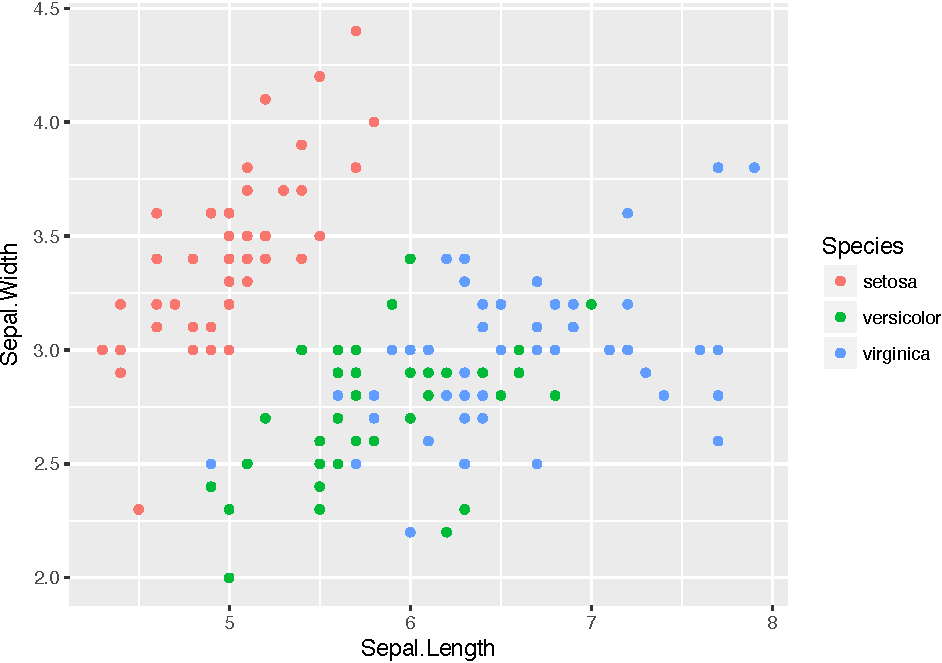
\includegraphics[width=0.9\linewidth]{bookdown_files/figure-latex/hello-1} \caption{Hello World!}\label{fig:hello}
\end{figure}

\begin{Shaded}
\begin{Highlighting}[]
\NormalTok{knitr::}\KeywordTok{kable}\NormalTok{(}
  \KeywordTok{head}\NormalTok{(iris), }\DataTypeTok{caption =} \StringTok{'The boring iris data.'}\NormalTok{,}
  \DataTypeTok{booktabs =} \OtherTok{TRUE}
\NormalTok{)}
\end{Highlighting}
\end{Shaded}

\begin{table}

\caption{\label{tab:iris}The boring iris data.}
\centering
\begin{tabular}[t]{rrrrl}
\toprule
Sepal.Length & Sepal.Width & Petal.Length & Petal.Width & Species\\
\midrule
5.1 & 3.5 & 1.4 & 0.2 & setosa\\
4.9 & 3.0 & 1.4 & 0.2 & setosa\\
4.7 & 3.2 & 1.3 & 0.2 & setosa\\
4.6 & 3.1 & 1.5 & 0.2 & setosa\\
5.0 & 3.6 & 1.4 & 0.2 & setosa\\
5.4 & 3.9 & 1.7 & 0.4 & setosa\\
\bottomrule
\end{tabular}
\end{table}

More chapters to come in \texttt{02-foo.Rmd}, \texttt{03-bar}.Rmd,
\ldots{}

\chapter{Evolutionary Genetics}\label{evolutionary-genetics}

\section{Evolution of genetic
systems}\label{evolution-of-genetic-systems}

\section{Phylogenetics}\label{phylogenetics}

\section{Game Theory}\label{game-theory}

\section{Genetic Algorithms}\label{genetic-algorithms}

\section{Evolutionary Algorithms}\label{evolutionary-algorithms}

\chapter{Population Genetics}\label{population-genetics}

\section{Hardy-Weinberg}\label{hardy-weinberg}

\section{Linkage Disequilibrium}\label{linkage-disequilibrium}

\chapter{Quantitative Genetics}\label{quantitative-genetics}

\section{QTL analysis}\label{qtl-analysis}

Quantitative Trait Loci (QTL) are regions in the genome that are
associated with variation in a quantitative trait. Quantitative traits
are phentoypes that can be measured on a continuous scale, like height,
weight, etc.

QTL analysis (or QTL mapping) is typically done on experimental
populations to find genes which contribute to the heritability of
traits. Phenotype and genetic marker data are collected from every
individual in the population. The general concept of QTL mapping is that
we can then calculate the correlation between genotypes and phenotypes
at each marker position and test whether they show a statistically
significant association.

Let's consider the famous example of \citet{Doebley285}, who assessed
the variation of traits that discriminate commercial maize from its
native relative teosinte. Teosinte is much smaller than maize as we know
it today and one teosinte plant produces many ears, each of which has
only two rows of seeds. But even though maize and teosinte look so
completely different, they are still able to produce viable offspring
together. \citet{Doebley285} utilized this and crossed the two plant
species to produce an F1 generation, which were in turn self-pollinated.
The resulting F2 population of maize-teosinte-hybrids showed a wide
range of intermediate parental morphologies. Each of the F2 offspring
was then genotyped at 58 locations in the genome, so that the
quantitative trait information on morphology could be correlated with
the genetic map. This analysis revealed that most of the morphological
variation between maize and teosinte were the result of changes in only
a handful of genes, one of which is the \emph{tb1} (\emph{teosinte
branched 1}) gene.

\subsection{Recombinant Inbred Lines
(RILs)}\label{recombinant-inbred-lines-rils}

RILs are experimental sister populations that have been produced by a
very specific back-crossing scheme. The process is similar to Doebley
and Stec's crossing of maize and teosinte: two homozygous parents are
crossed to produce an F1 generation. Following the laws of genetics,
each offspring's genome consists of a random combination of parental
alleles and crossover (or recombination) events. Depending on the
design, F1 offspring are usually either selfed or mated with a sibling
to introduce another level of genetic recombination. The final
generation is then inbred for many generations to obtain a collection of
homozygous sister lines, each with a unique mosaic genome of parental
alleles \citep{Pollard2012}.

\subsection{QTL analysis in R}\label{qtl-analysis-in-r}

\subsubsection{\texorpdfstring{The ``qtl''
package}{The qtl package}}\label{the-qtl-package}

The best established R package for QTL mapping is Karl Broman's
\href{http://www.rqtl.org/}{\textbf{qtl} package} \citep{R-qtl}. It
implements several techniques for finding QTLs, like Hidden Markov
Models (HMM), interval mapping, Haley-Knott regression and multiple
imputation. It is very well documented and comes with extensive example
data and code.

Here, I will introduce you to a basic QTL mapping workflow using the
examples given in the package documentation and refer you to more
complex analysis options where applicable.

\paragraph*{Installation and loading the
package}\label{installation-and-loading-the-package}
\addcontentsline{toc}{paragraph}{Installation and loading the package}

If this is the first time you are using the \textbf{qtl} package, you
need to install it from CRAN. The following line of code checks whether
you already have the package, and if not installs it.

\begin{Shaded}
\begin{Highlighting}[]
\NormalTok{pkg =}\StringTok{ "qtl"}
\NormalTok{if (}\KeywordTok{system.file}\NormalTok{(}\DataTypeTok{package =} \NormalTok{pkg) ==}\StringTok{ ''}\NormalTok{) }\KeywordTok{install.packages}\NormalTok{(pkg)}
\end{Highlighting}
\end{Shaded}

You can then load the package:

\begin{Shaded}
\begin{Highlighting}[]
\KeywordTok{library}\NormalTok{(qtl)}
\end{Highlighting}
\end{Shaded}

\paragraph*{Loading the data}\label{loading-the-data}
\addcontentsline{toc}{paragraph}{Loading the data}

I will be using the example data on murine hypertension that is provided
in the package \citep{Sugiyama200170}. The \textbf{summary()} function
shows you the main properties of the data:

\begin{Shaded}
\begin{Highlighting}[]
\KeywordTok{data}\NormalTok{(hyper)}
\KeywordTok{summary}\NormalTok{(hyper)}
\end{Highlighting}
\end{Shaded}

\begin{verbatim}
##     Backcross
## 
##     No. individuals:    250 
## 
##     No. phenotypes:     2 
##     Percent phenotyped: 100 100 
## 
##     No. chromosomes:    20 
##         Autosomes:      1 2 3 4 5 6 7 8 9 10 11 12 13 
##                         14 15 16 17 18 19 
##         X chr:          X 
## 
##     Total markers:      174 
##     No. markers:        22 8 6 20 14 11 7 6 5 5 14 5 5 
##                         5 11 6 12 4 4 4 
##     Percent genotyped:  47.7 
##     Genotypes (%):    
##           Autosomes:    BB:50.1  BA:49.9 
##        X chromosome:    BY:53.0  AY:47.0
\end{verbatim}

The \textbf{plot()} function produces plots showing missing genotypes,
the marker positions and the distribution of phenotypes or traits. This
will give you a first idea of your data.

The \href{http://www.rqtl.org/tutorials/rqtltour.pdf}{package manual}
includes a description of various additional plotting functions, which I
won't cover here. I also advise to examine each object with
\textbf{head()} or \textbf{summary()} after you ran a function to get a
feel for your data and the various steps you are taking in the analysis.

\begin{Shaded}
\begin{Highlighting}[]
\KeywordTok{plot}\NormalTok{(hyper)}
\end{Highlighting}
\end{Shaded}

\begin{center}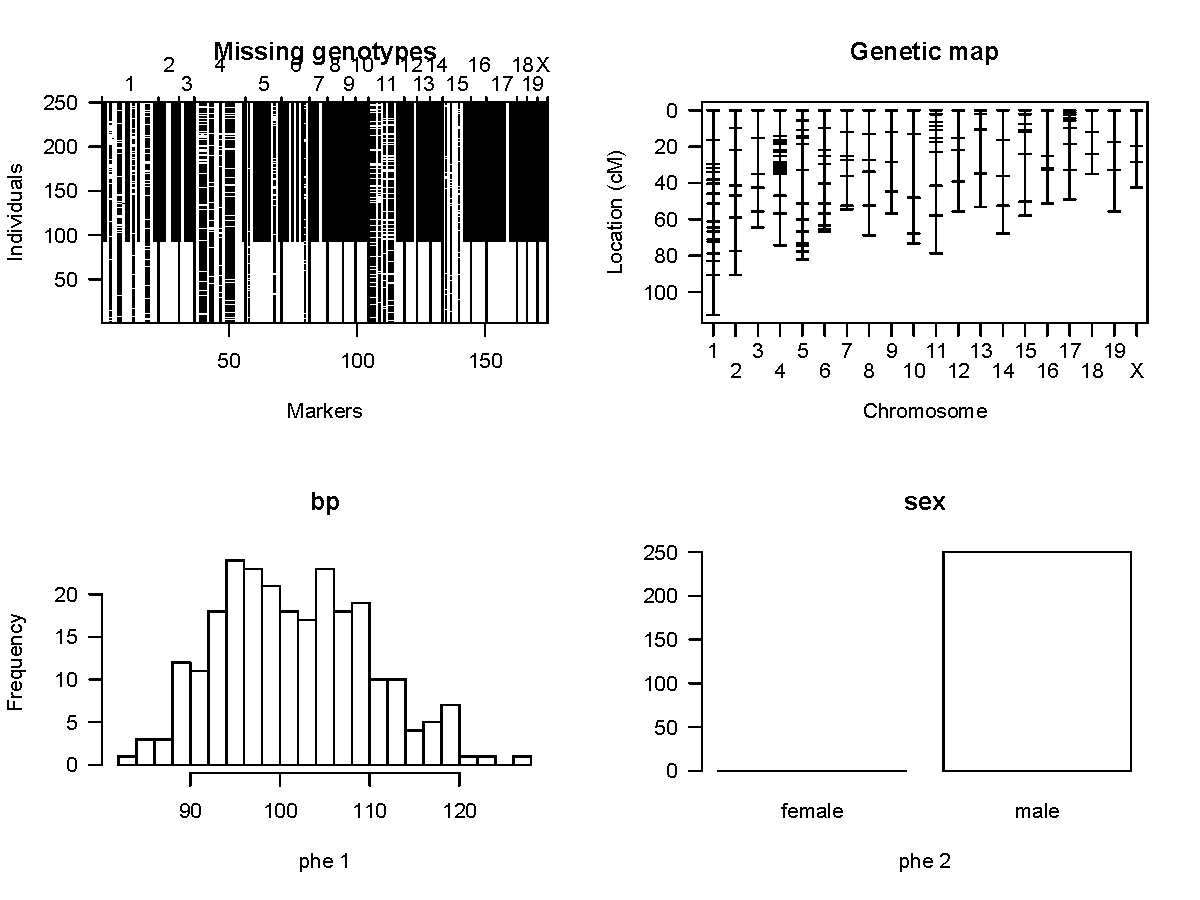
\includegraphics{bookdown_files/figure-latex/unnamed-chunk-6-1} \end{center}

\paragraph*{Genetic map estimation}\label{genetic-map-estimation}
\addcontentsline{toc}{paragraph}{Genetic map estimation}

Before we proceed with the analysis, I typically recommend to replace
the existing genetic map with an estimated one to reduce the potential
errors. The genetic map represents all markers on a chromosome in a
linear fashion. The \textbf{est.map()} function applies a Hidden Markov
Model \citep{Lander01041987} to estimate the map with an assumed
genotyping error rate (\emph{error.prob}).

Here, we can also specify the mapping function (\emph{map.function})
that we want to use to convert genetic distance to recombination
fraction. The distance between two markers is usually given as a unit of
genetic linkage, called \emph{centimorgan (cM)} One cM represents the
distance with an average of 0.01 crossover events in one generation
(i.e.~1\% recombination). However, this representation of distance
underestimates the actual recombination fraction, which is inherently
not additive. With increasing distance the chance of double crossovers
increases, so that they are in a way ``invisible'' to the traditional
estimation of recombination distance.

Another reason why genetic maps based on recombination are biased is
crossover interference, which described the phenomenon that a crossover
event reduces the likelihood of another recombination event occur close
by.

To correct for such biases, we can choose from the following mapping
functions:

\begin{itemize}
\tightlist
\item
  \textbf{Haldane's} is the simplest mapping function and assumes a
  Poisson distribution for crossover events and does not consider
  interference.
\item
  \textbf{Kosambi's} mapping function also considers interference and
  double crossovers but it can not calculate joint recombination
  probabilities for more than three loci.
\item
  \textbf{Carter-Falconer's} mapping function can be extended to more
  complex interference rates.
\item
  \textbf{Morgan's} mapping function assumes complete interference.
\end{itemize}

The two most widely used mapping functions are Haldane's (the default)
and Kosambi's. For this example, using Haldane's should be sufficient.
Because our example is a backcross, we can assume no interference,
meaning that all crossovers are independent \citep{lynch1998genetics}.

\begin{Shaded}
\begin{Highlighting}[]
\NormalTok{newmap <-}\StringTok{ }\KeywordTok{est.map}\NormalTok{(hyper, }\DataTypeTok{error.prob =} \FloatTok{0.0001}\NormalTok{, }\DataTypeTok{map.function =} \StringTok{"haldane"}\NormalTok{)}
\NormalTok{hyper <-}\StringTok{ }\KeywordTok{replace.map}\NormalTok{(hyper, newmap)}
\end{Highlighting}
\end{Shaded}

We can now estimate the recombination fractions between all pairs of
markers. The \textbf{est.rf()} function also calculates the LOD scores.
LOD stands for ``likelihood of the odds'' and is a measure of linkage.
In QTL mapping we calculate LOD scores for the genetic markers and a
threshold, above which we consider a QTL statistically significant in
its association with the trait.

\begin{Shaded}
\begin{Highlighting}[]
\NormalTok{hyper <-}\StringTok{ }\KeywordTok{est.rf}\NormalTok{(hyper)}
\end{Highlighting}
\end{Shaded}

The \textbf{calc.errorlod()} function calculates the genotyping errors
according to \citet{Lincoln1992604}. We can see which markers have an
error LOD above a certain threshold (cutoff) with the
\textbf{top.errorlod()} function.

\begin{Shaded}
\begin{Highlighting}[]
\NormalTok{hyper <-}\StringTok{ }\KeywordTok{calc.errorlod}\NormalTok{(hyper, }\DataTypeTok{error.prob =} \FloatTok{0.0001}\NormalTok{)}
\NormalTok{te <-}\StringTok{ }\KeywordTok{top.errorlod}\NormalTok{(hyper, }\DataTypeTok{cutoff =} \DecValTok{3}\NormalTok{)}
\NormalTok{te}
\end{Highlighting}
\end{Shaded}

\begin{verbatim}
##   chr  id   marker errorlod
## 1   4 102 D4Mit288    3.325
## 2   4 107 D4Mit111    3.262
## 3   4 216 D4Mit214    3.261
## 4  11  57 D11Mit82    3.021
## 5  11 118 D11Mit82    3.021
\end{verbatim}

\begin{Shaded}
\begin{Highlighting}[]
\NormalTok{hyper.clean <-}\StringTok{ }\NormalTok{hyper}
\NormalTok{for(i in }\DecValTok{1}\NormalTok{:}\KeywordTok{nrow}\NormalTok{(te)) \{}
  \NormalTok{chr <-}\StringTok{ }\NormalTok{te$chr[i]}
  \NormalTok{id <-}\StringTok{ }\NormalTok{te$id[i]}
  \NormalTok{mar <-}\StringTok{ }\NormalTok{te$marker[i]}
  \NormalTok{hyper.clean$geno[[chr]]$data[hyper$pheno$id ==}\StringTok{ }\NormalTok{id, mar] <-}\StringTok{ }\OtherTok{NA}
\NormalTok{\}}
\end{Highlighting}
\end{Shaded}

\paragraph*{Finding QTLs}\label{finding-qtls}
\addcontentsline{toc}{paragraph}{Finding QTLs}

Now, we can proceed with the central step: mapping the QTLs.

Because the individuals in QTL studies are genotyped at specific marker
locations throughout the genome, we inherently have to deal with the
missing information about genotypes between markers. Hidden Markov
Models (HMM) can help us overcome this problem by calculating genotype
probabilities between markers based on the joint genotype distribution.

We first need to calculate these genotype probabilities using the
\textbf{calc.genoprob()} function. We can define several parameters,
like step size, the amount of error we want to allow for, the mapping
function and step width. Here, we want to calculate genotype
probabilities for every cM (step = 1), with a fixed step width and an
error probability of 0.0001. As above, we are again using Haldane's
mapping function.

\begin{Shaded}
\begin{Highlighting}[]
\NormalTok{hyper.clean <-}\StringTok{ }\KeywordTok{calc.genoprob}\NormalTok{(hyper.clean, }\DataTypeTok{step =} \DecValTok{1}\NormalTok{, }\DataTypeTok{error.prob =} \FloatTok{0.0001}\NormalTok{, }\DataTypeTok{map.function =} \StringTok{"haldane"}\NormalTok{, }\DataTypeTok{stepwidth =} \StringTok{"fixed"}\NormalTok{)}
\end{Highlighting}
\end{Shaded}

The simplest QTL model, we can run is single-QTL marker regression or
interval mapping using the \textbf{scanone()} function.

These simple methods can give a good estimation of QTLs but they can
also introduce bias, especially with multiple QTL in close proximity.
More advanced mapping approaches, like Composite Interval Mapping (CIM)
are discussed later on.

The first parameter we want to specify is the phenotype(s) and model
(e.g.~parametric or non-parametric) for mapping. Here, we want to use
the first phenotype, i.e.~the first column in our phenotype matrix,
which follows a normal distribution. We can see the phenotype matrix by
calling:

\begin{Shaded}
\begin{Highlighting}[]
\NormalTok{hyper.clean$pheno}
\end{Highlighting}
\end{Shaded}

Then, we need to specify the mapping algorithm we want to use. We can
choose from several options. Here, I will only present the practical
implications for each method. For a full discussion of the mathematical
principles, see \citet{lynch1998genetics}.

\begin{itemize}
\tightlist
\item
  \textbf{Marker regression}: Marker regression is by far the simplest
  approach to QTL mapping. Here, we calculate the association between
  phenotype and genotype at each marker position independently.
\end{itemize}

Because it is so simple, marker regression is seldom recommended to use.
With interval mapping, a phenotype \textasciitilde{} genotype
association analysis is performed for each flanking marker pair
independently. This improves the approximation and gives confidence
regions around QTL.

\begin{itemize}
\tightlist
\item
  \textbf{EM (Expectation-Maximization) algorithm}: EM is usually
  applied to maximum likelihood (ML) analyses of mixed models. It is an
  iterative process of calculating conditional probabilities and
  updating the ML estimates. This process is repeated until the
  estimates converge \citep{Lander185}. If we have a reasonably dense
  marker map, the EM algorithm will converge on the global maximum.
\item
  \textbf{(Extended) Haley-Knott regression}: Haley-Knott regression
  uses a simpler model than the EM algorithm \citep{Haley1992}. The
  extended Haley-Knott regression also considers variance is therefore
  gives improved approximations. Haley-Knott regression can give good
  approximations of the likelihood profiles for ML interval mapping but
  with more complex cases, it can be heavily biased.
\item
  \textbf{Multiple imputation}: This method uses multiple rounds of
  imputing the unknown genotypes between markers and combines them into
  a final imputation model \citep{Sen371}. This allows us to perform a
  simple analysis of variance at each position in the genome. Multiple
  imputation needs much more computational power than simpler methods
  and will usually not outperform them with single-QTL models (it is
  much more advantageous with more complex multi-QTL models, however).
\end{itemize}

Here, I will show QTL mapping examples for the EM algorithm and for
multiple imputation:

\begin{Shaded}
\begin{Highlighting}[]
\CommentTok{# EM algorithm}
\NormalTok{out.em <-}\StringTok{ }\KeywordTok{scanone}\NormalTok{(hyper.clean, }\DataTypeTok{pheno.col =} \DecValTok{1}\NormalTok{, }\DataTypeTok{model =} \StringTok{"normal"}\NormalTok{, }\DataTypeTok{method =} \StringTok{"em"}\NormalTok{)}
\end{Highlighting}
\end{Shaded}

The multiple imputation method requires the use of the
\textbf{sim.geno()} function before we call the mapping function. It
calculates the joint genotype distribution based on the available marker
information and uses it to perform the imputation of missin genotypes.
With the \textbf{n.draws} parameter, we define how many imputations will
be run. The more imputations steps we run, the more precise the
genotypes but with increasing cost of computational time and power.

\begin{Shaded}
\begin{Highlighting}[]
\NormalTok{hyper.clean <-}\StringTok{ }\KeywordTok{sim.geno}\NormalTok{(hyper.clean, }\DataTypeTok{step =} \DecValTok{1}\NormalTok{, }\DataTypeTok{n.draws =} \DecValTok{100}\NormalTok{, }\DataTypeTok{error.prob =} \FloatTok{0.0001}\NormalTok{, }\DataTypeTok{map.function =} \StringTok{"haldane"}\NormalTok{, }\DataTypeTok{stepwidth =} \StringTok{"fixed"}\NormalTok{)}
\NormalTok{out.imp <-}\StringTok{ }\KeywordTok{scanone}\NormalTok{(hyper.clean, }\DataTypeTok{pheno.col =} \DecValTok{1}\NormalTok{, }\DataTypeTok{model =} \StringTok{"normal"}\NormalTok{, }\DataTypeTok{method =} \StringTok{"imp"}\NormalTok{)}
\end{Highlighting}
\end{Shaded}

Now that we have a LOD score for each marker position, we want to know
which positions are significantly associated with the phenotype. To
determine this, we will use the \textbf{scanone()} function again, but
this time we want to calculate the genome-wide LOD score threshold with
a permutation test. Above this threshold we can consider a QTL to be
statistically significant. Here, I am using a similar call as before,
but I am specifying that we want to use 1000 permutations.

\begin{Shaded}
\begin{Highlighting}[]
\NormalTok{operm.imp <-}\StringTok{ }\KeywordTok{scanone}\NormalTok{(hyper.clean, }\DataTypeTok{pheno.col =} \DecValTok{1}\NormalTok{, }\DataTypeTok{model =} \StringTok{"normal"}\NormalTok{, }\DataTypeTok{method =} \StringTok{"imp"}\NormalTok{, }\DataTypeTok{n.perm =} \DecValTok{1000}\NormalTok{)}
\end{Highlighting}
\end{Shaded}

\begin{verbatim}
## Doing permutation in batch mode ...
\end{verbatim}

The \textbf{summary()} function will tell us our genome-wide LOD score
threshold for a given significance value (here 0.05).

\begin{Shaded}
\begin{Highlighting}[]
\NormalTok{lod <-}\StringTok{ }\KeywordTok{summary}\NormalTok{(operm.imp, }\DataTypeTok{alpha =} \FloatTok{0.05}\NormalTok{)}
\NormalTok{lod}
\end{Highlighting}
\end{Shaded}

\begin{verbatim}
## LOD thresholds (1000 permutations)
##     lod
## 5% 2.28
\end{verbatim}

And now we can also refine our QTL results by including the significance
threshold. This will give us the LOD score and estimated p-values for
each marker above the threshold, around which we can now assume to have
found a QTL for our trait of interest.

\begin{Shaded}
\begin{Highlighting}[]
\KeywordTok{summary}\NormalTok{(out.imp, }\DataTypeTok{perms =} \NormalTok{operm.imp, }\DataTypeTok{alpha =} \FloatTok{0.05}\NormalTok{, }\DataTypeTok{pvalues =} \OtherTok{TRUE}\NormalTok{)}
\end{Highlighting}
\end{Shaded}

\begin{verbatim}
##           chr   pos  lod  pval
## c1.loc98    1 101.3 3.74 0.001
## D4Mit164    4  41.6 8.09 0.000
## D15Mit152  15  37.3 2.34 0.043
\end{verbatim}

Now that we have our QTL, we can plot them with the \textbf{plot()}
function. Here, I am plotting the results from both, the EM algorithm
and the multiple imputation method. As expected, they do not differ
much. The horizontal dotted line shows the genome-wide LOD threshold and
our two significant QTL pop up nicely on chromosomes 1 and 4.

\begin{Shaded}
\begin{Highlighting}[]
\KeywordTok{plot}\NormalTok{(out.em, }\DataTypeTok{col =} \StringTok{"blue"}\NormalTok{)}
\KeywordTok{plot}\NormalTok{(out.imp, }\DataTypeTok{col =} \StringTok{"red"}\NormalTok{, }\DataTypeTok{add =} \OtherTok{TRUE}\NormalTok{)}
\KeywordTok{abline}\NormalTok{(}\DataTypeTok{h =} \NormalTok{lod[}\DecValTok{1}\NormalTok{], }\DataTypeTok{lty =} \DecValTok{2}\NormalTok{)}
\KeywordTok{legend}\NormalTok{(}\StringTok{"topright"}\NormalTok{, }\KeywordTok{c}\NormalTok{(}\StringTok{"EM algorithm"}\NormalTok{,}\StringTok{"Mult. imputation"}\NormalTok{), }\DataTypeTok{col =} \KeywordTok{c}\NormalTok{(}\StringTok{"blue"}\NormalTok{, }\StringTok{"red"}\NormalTok{), }\DataTypeTok{lty =} \DecValTok{1}\NormalTok{, }\DataTypeTok{lwd =} \DecValTok{3}\NormalTok{)}
\end{Highlighting}
\end{Shaded}

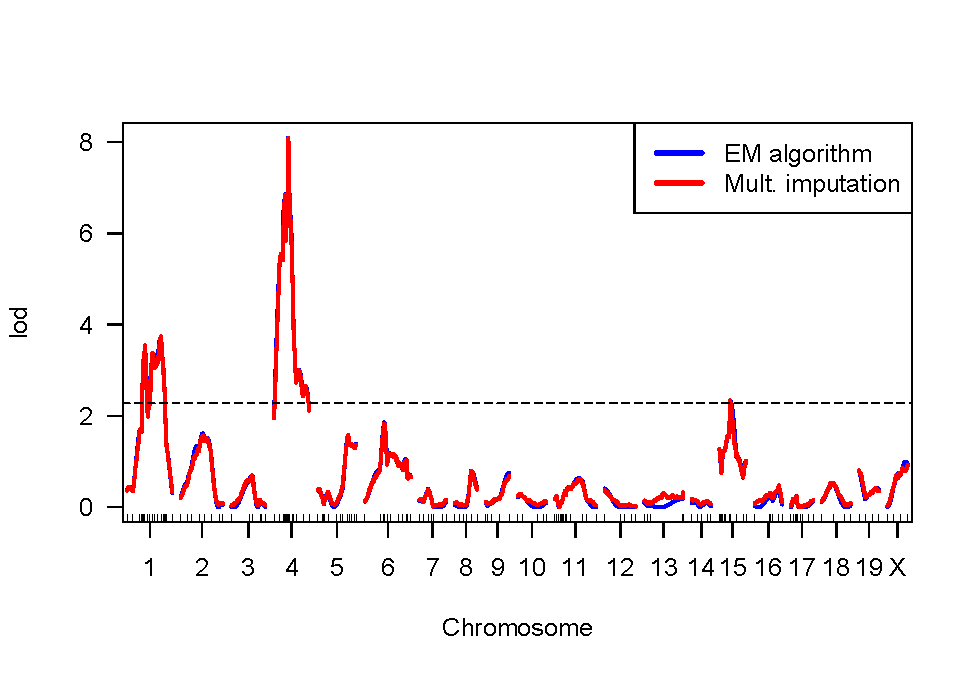
\includegraphics{bookdown_files/figure-latex/unnamed-chunk-18-1.pdf}

\paragraph*{QTL interaction mapping}\label{qtl-interaction-mapping}
\addcontentsline{toc}{paragraph}{QTL interaction mapping}

\paragraph*{Covariates in QTL models}\label{covariates-in-qtl-models}
\addcontentsline{toc}{paragraph}{Covariates in QTL models}

\subsubsection{\texorpdfstring{QTL Analysis using Bayesian Interval
Mapping (``qtlbim''
package)}{QTL Analysis using Bayesian Interval Mapping (qtlbim package)}}\label{qtl-analysis-using-bayesian-interval-mapping-qtlbim-package}

\section{Gene x Environment
interactions}\label{gene-x-environment-interactions}

\section{Variance and heritability}\label{variance-and-heritability}

\chapter{Genetics of complex
diseases}\label{genetics-of-complex-diseases}

\section{Genome Wide Association Studies
(GWAS)}\label{genome-wide-association-studies-gwas}

\section{Pedigree analysis}\label{pedigree-analysis}

\chapter{Genetic Epidemiology}\label{genetic-epidemiology}

\section{Infection models}\label{infection-models}

\cleardoublepage 

\appendix \addcontentsline{toc}{chapter}{\appendixname}


\chapter{More to Say}\label{more-to-say}

Yeah! I have finished my book, but I have more to say about some topics.
Let me explain them in this appendix.

To know more about \textbf{bookdown}, see \url{https://bookdown.org}.

\bibliography{packages,book}

\backmatter
\printindex

\end{document}
